% Imported from topics/video-generation/seedance-2.5/architecture.md
\chapter{Wan 基座的增量候选架构}\label{seedance-m12}
\moduleinfo{M12}{增量路线与工程阅读；未运行教学代码}{\hyperref[src-wan-2.1]{\texttt{wan-2.1}}、\hyperref[src-seedance-1.0]{\texttt{seedance-1.0}}、\hyperref[src-phantom]{\texttt{phantom}}、\hyperref[src-long-context-tuning]{\texttt{long-context-tuning}}、\hyperref[src-seedance-2.5-release]{\texttt{seedance-2.5-release}}、\hyperref[src-wan21-code]{\texttt{wan21-code}}、\hyperref[src-diffsynth-code]{\texttt{diffsynth-code}}、\hyperref[src-phantom-code]{\texttt{phantom-code}}、\hyperref[src-longlive-code]{\texttt{longlive-code}}、\hyperref[src-ltx-code]{\texttt{ltx-code}}}

前文主线使用联合音视频基座；这一章另列 Wan 视频单项路线，便于较小规模的机制与适配试验。

前面分别讨论了参考、编辑和长视频，现在尝试把它们接到一个可获得的基座上。先取 Wan-2.1 T2V-1.3B，保留已训练的接口，再逐步增加条件。这样能明确每一步修改了哪里。下面是一套待实验的增量设计，不据此认定它就是 Seedance 2.5 的内部结构。

这条路线适合先研究视频单项能力，音轨可通过后期流程制作。需要在一个主干内联合处理声音、多参考、编辑和长叙事时，另有以 LTX-2 原系列为基础的 \hyperref[seedance-m19]{完整候选架构} 与 \hyperref[seedance-m20]{联合训练配方}；两条路线分别维护潜空间、权重和训练配置。

\section{先保留基座的有效接口}\label{seedance-m12-ux5148ux4fddux7559ux57faux5ea7ux7684ux6709ux6548ux63a5ux53e3}

Wan 的 VAE 使用时间四倍、空间八倍压缩，潜变量为 16 通道；DiT 再采用 \codepath{1×2×2} patch，文本由 umT5 编码并通过交叉注意力进入视觉主干。

\begin{figure}
\centering
\pandocbounded{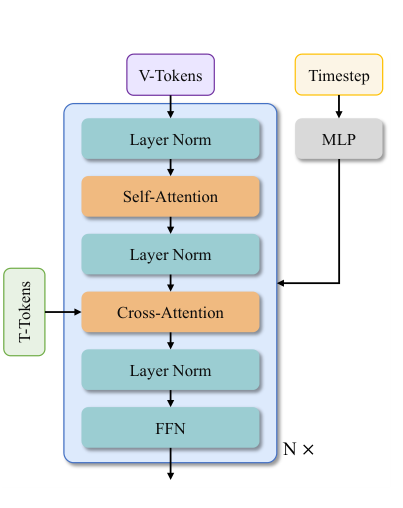
\includegraphics[keepaspectratio,alt={基座的视觉自注意力、文本交叉注意力与前馈模块 （论文示意，来源：wan-2.1）}]{assets/seedance/figures/wan-block.png}}
\caption{基座的视觉自注意力、文本交叉注意力与前馈模块 （论文示意，来源：wan-2.1）}
\end{figure}

先保留这些接口，是因为原权重已经在相应潜变量和文本特征上训练过。另一种 VAE 即使输出相似网格，通道意义、分布和归一化也可能不同；换文本编码器、patch 或位置布局也一样。张量能拼上，还不能说明权重仍在处理它认识的数据。

1.3B 相对适合缩小实验，但推理能运行不等于全参训练资源足够。开始前仍需固定源码、checkpoint、许可证、依赖和硬件基线，再测量实际显存与吞吐。

\section{请求先编译成任务}\label{seedance-m12-ux8bf7ux6c42ux5148ux7f16ux8bd1ux6210ux4efbux52a1}

任务先从用户语言翻译成可计算的条件：主体、镜头、时间、参考用途、必须保持与允许变化的内容。原始要求另外保存，再生成稠密提示，才能检查人数、动作顺序和否定条件有没有在改写中改变。

\begin{verbatim}
用户要求与素材
  → 任务解析与约束检查
  → 素材绑定、参考编码、文本编码
  → 带条件的视频采样
  → VAE 解码、局部合成、音轨处理
  → 自动检查与人工审片
  → 交付或定向返工
\end{verbatim}

如果角色指代或时间尚不明确，后面就没有唯一的绑定对象。缺素材、绑定互相冲突，也应在生成前显式解决，不能把不确定性藏进模型输入，再将模型忽略条件当成一次普通失败。

\section{参考支路怎样增加}\label{seedance-m12-ux53c2ux8003ux652fux8defux600eux6837ux589eux52a0}

先只加入图片身份与外观参考。图片经过基座 VAE、投影和定额池化，形成 \codepath{B,R,d_ref} 的参考记忆；每个 token 携带 role、subject、shot 和时间信息。

在部分主干层后加入门控交叉注意力：

\[
h'_v=h_v+g\operatorname{Attn}(Q_v,K_r,V_r).
\]

插入密度先取每四个 Transformer block 一次，门控零初始化，主干冻结，只训练新支路。这样先看这条路径本身能否学习。随后再比较更密或更疏的插入、不同 token 预算，以及有限 LoRA 解冻；这组初值不是已经证明的最优解。

参考按镜头检索与分配预算，初期可试总计 1024 个 token，同时保留更高预算对照。超额时记录截断项；精细 logo、多人身份和动作视频可能需要不同的编码与预算。

\section{局部编辑为什么另加条件路径}\label{seedance-m12-ux5c40ux90e8ux7f16ux8f91ux4e3aux4ec0ux4e48ux53e6ux52a0ux6761ux4ef6ux8defux5f84}

T2V checkpoint 本身没有自动长出源视频和区域 mask 的接口。编辑因而需要新增源条件支路，读取源 latent、编辑与上下文 mask，再以残差影响主干。目标原来的带噪输入通道先保留，避免新增条件时把旧输入头的权重关系一起改掉。

生成后的局部区域与源帧合成，可使不允许变化的位置直接复用原像素。若目标是姿态或视角变化，则另定义语义与几何保持条件，不能继续使用逐像素不变作为唯一标准。

参考与源条件先分开训练，再分别观察结果。否则身份没保持，可能是参考没有读到，也可能是编辑任务改变了它；两条路径同时变化，就不容易定位原因。

\section{多镜头先编排，再研究原生长上下文}\label{seedance-m12-ux591aux955cux5934ux5148ux7f16ux6392ux518dux7814ux7a76ux539fux751fux957fux4e0aux4e0bux6587}

多镜头也可以从更小的问题开始：先用角色资产和状态记录连接几个短镜头，再显式剪辑。外观、道具归属、位置以及已经发生的事件，都是下一镜头的条件，而不只是给编辑器看的附注。

等短镜头控制可靠，再尝试场景级联合训练和因果续写。前者涉及逐镜头噪声时间，后者还涉及固定历史与缓存失效。它们改变了模型读到什么，不能通过给原输入增加一个长序列参数就得到。

多镜头编排形成三十秒成片，与原生一次生成三十秒，属于不同成果，应使用不同的质量、成本和局部修改标准。

\section{音频与服务层怎样安排}\label{seedance-m12-ux97f3ux9891ux4e0eux670dux52a1ux5c42ux600eux6837ux5b89ux6392}

起步版本可以独立配音、制作音效并确定性混流。强口型或动作音效同步任务，再单独引入音频 codec、音频主干与联合训练；需要对齐数据、语言覆盖和同步验证。

媒体与 latent 放对象存储，任务数据库保存版本和依赖。CPU 解码、GPU 描述与编码、训练、推理分别成为 worker；小规模用本地 manifest 和简单队列即可，吞吐成为瓶颈后再增加分布式调度。

每次输出应能反查模型、适配器、数据、提示、参考、种子和 scheduler。用户再次生成只是行为信号，需结合失败标注才能进入训练反馈。

\section{用阶段门槛控制复杂度}\label{seedance-m12-ux7528ux9636ux6bb5ux95e8ux69dbux63a7ux5236ux590dux6742ux5ea6}

{\def\LTcaptype{table} % do not increment counter
\small\setlength{\tabcolsep}{3pt}\renewcommand{\arraystretch}{1.18}
\begin{longtable}[]{@{}
  >{\raggedright\arraybackslash}p{(\linewidth - 2\tabcolsep) * \real{0.2200}}
  >{\raggedright\arraybackslash}p{(\linewidth - 2\tabcolsep) * \real{0.7800}}@{}}
\toprule\noalign{}
\begin{minipage}[b]{\linewidth}\raggedright
阶段
\end{minipage} & \begin{minipage}[b]{\linewidth}\raggedright
需要证明的结果
\end{minipage} \\
\midrule\noalign{}
\endhead
\bottomrule\noalign{}
\endlastfoot
原版基线 & 短片生成、VAE 重建、计时与重复运行正确 \\
图片参考 & 一到四图较纯文本改善身份，动作不过度退化 \\
区域编辑 & 目标变化、非目标保持、时间边界稳定 \\
多镜头 & 角色与道具状态在两到四镜头间持续成立 \\
原生长上下文 & 长 rollout 稳定，缓存与重算等价 \\
联合音频 & 同步、音质和视频质量共同达到任务标准 \\
\end{longtable}
}

这样分阶段，目的是让每项能力有可观察的任务和退出条件。某条路线暂时没有收益，还能保留已经验证的部件；如果只以架构图是否完整为目标，未解决的依赖就会一路进入后续系统。

\section{真实工程从哪里进入}\label{seedance-m12-ux771fux5b9eux5de5ux7a0bux4eceux54eaux91ccux8fdbux5165}

基础生成选 \href{https://github.com/Wan-Video/Wan2.1}{Wan}，训练入口选 \href{https://github.com/modelscope/DiffSynth-Studio}{DiffSynth}，参考推理看 \href{https://github.com/Phantom-video/Phantom}{Phantom-Wan}，长视频单独看 \href{https://github.com/NVlabs/LongLive/blob/31c70d9071cd7851d82939806dc9fac645fcabe5/LongLive1.0/inference.py}{LongLive1.0}，联合音视频另走 \href{https://github.com/Lightricks/LTX-2}{LTX}。每条路线的固定版本、接口差异和代码入口列在 \hyperref[seedance-m15]{代码路线与仓库选择}；本地只保留讲机制的极简片段，不另搭一个训练框架。
